% Suggested time: 1.3 minutes
\begin{frame}[t]{Masking decides which trace tokens create gradients}
  \begin{columns}[T,onlytextwidth]
    \begin{column}{0.38\textwidth}
      \centering
      \begin{tikzpicture}[node distance=1.5mm]
        \node[flowbox,text width=42mm,minimum height=8mm,inner sep=1mm] (system)
          {\textbf{System}\quad \textcolor{DeckMuted}{$m=0$: masked}\\[-1mm]
           \scriptsize coding-agent instructions};
        \node[flowbox,text width=42mm,minimum height=8mm,inner sep=1mm,below=of system] (user)
          {\textbf{User}\quad \textcolor{DeckMuted}{$m=0$: masked}\\[-1mm]
           \scriptsize ``Check port 3000''};
        \node[signalbox,text width=42mm,minimum height=8mm,inner sep=1mm,below=of user] (assistant1)
          {\textbf{Assistant}\quad $m=1$: loss\\[-1mm]
           \scriptsize call \texttt{curl 3000}};
        \node[warnbox,text width=42mm,minimum height=8mm,inner sep=1mm,below=of assistant1] (tool)
          {\textbf{Tool result}\quad \textcolor{DeckMuted}{$m=0$ default}\\[-1mm]
           \scriptsize \textcolor{DeckRed}{ECHO adds loss}\quad \texttt{not\_found}};
        \node[signalbox,text width=42mm,minimum height=8mm,inner sep=1mm,below=of tool] (assistant2)
          {\textbf{Assistant}\quad $m=1$: loss\\[-1mm]
           \scriptsize choose the next action};
        \draw[flowarrow] (system) -- (user);
        \draw[flowarrow] (user) -- (assistant1);
        \draw[flowarrow] (assistant1) -- (tool);
        \draw[flowarrow] (tool) -- (assistant2);
      \end{tikzpicture}

      \vspace{0.5mm}
      {\scriptsize \textbf{Default SFT:} assistant-only loss.}
    \end{column}
    \begin{column}{0.59\textwidth}
      \centering
      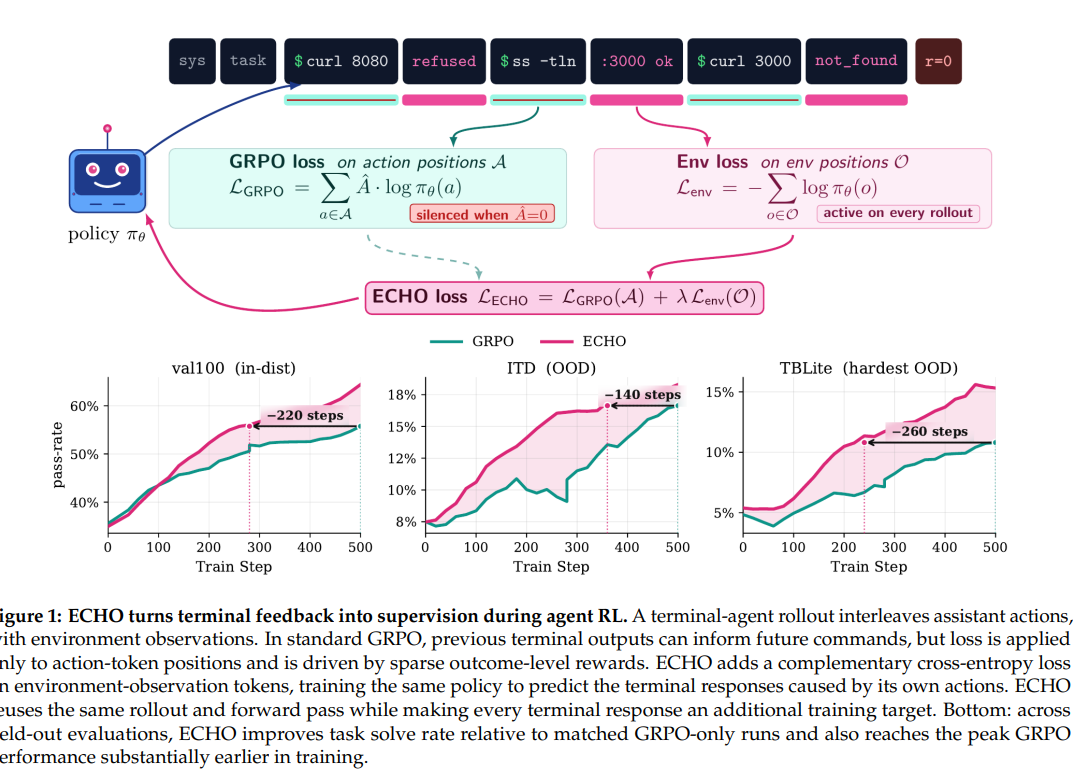
\includegraphics[width=\textwidth,height=0.59\textheight,keepaspectratio,
        trim=0 145 0 0,clip]{figures/ECHO_Loss.png}

      \vspace{1mm}
      {\scriptsize ECHO also trains environment/tool-result tokens, improving pass rate in its experiments \citep{shrivastava2026echo}.}
    \end{column}
  \end{columns}
\end{frame}
